\section{Diskussion}
\label{sec:Diskussion}

Die in den Abbildungen \ref{fig:duenn30}, \ref{fig:mittel30} und \ref{fig:dick30} dargestellten Kurven zeigen eine lineare Abhängigkeit zwischen der Frequenzverschiebung durch den Dopplerwinkel im Vergleich zur bestimmten Strömungsgeschwindigkeit.
Dies heißt, dass bei geringeren Strömungsgeschwindigkeiten eine geringere Frequenzverschiebung stattfindet.
Wird die Frequenzverschiebungen untereinander verglichen, so ergibt sich, dass die Messbereich für kleinere Rohrdurchmesser größer sind als für die größeren Rohrdurchmesser.

Die in den Abbildungen \ref{fig:v1} und \ref{fig:v2} dargstellten Strömungsprofile zeigen die typischen Geschwindigkeitsverteilungen, wie man sie von einer laminaren Strömung erwarten würde.
Ein Vergleich zwischen einer laminaren und turbulenten Strömung ist in Abbildung \ref{fig:profil} dargestellt.

\begin{figure}
  \centering
  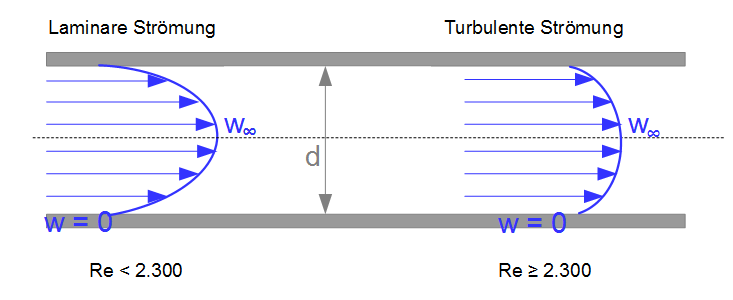
\includegraphics[width=\textwidth]{images/Stroemungsprofil.png}
  \caption{Vergleich zwischen turbulenter und laminarer Strömung \cite{profil}}
  \label{fig:v1}
\end{figure}

Es fällt allerdings auf, dass die Messwerte ab einer Eindringtiefe von $\SI{8}{\milli\metre}$ nicht mehr dem zu erwartendem Profil entsprechen.
Dies lässt sich damit erklären, dass diese Werte nicht mehr innerhalb des Rohres sind.
Die Streuintensität verhält sich entgegengesetzt zu den Geschwindigkeiten und ist für hohe Geschwindigkeiten geringer.
Dies leuchtet ein, da bei höheren Strömungsgeschwindigkeiten die Frequenzverschiebungen größer sind.
Das Spektrum der Frequenzverschiebungen ist breiter und Abweichungen vom Durschnitt weniger signifikant, die Streuintensität also geringer.
